\documentclass[10pt]{report}

\usepackage{geometry}
\geometry{
	letterpaper,
	hmargin=0.5in,
	vmargin=1in,
	footskip=0.25in
}

\usepackage{enumerate} % for enumerate counter
\usepackage{subcaption} % for subfigures
\usepackage{amsthm} % for QED
\usepackage{mathtools} % for delimiter

\usepackage{listings} % for code
\lstset{ 
	language=R,
	basicstyle=\footnotesize\ttfamily,
	numbers=none,
	stepnumber=1,
	numbersep=8pt,
	showspaces=false,
	showstringspaces=false,
	showtabs=false,
	frame=single,
	tabsize=2,
	captionpos=t,
	breaklines=true,
	breakatwhitespace=false
} 

\usepackage{float} % for figure [H]
\usepackage{booktabs} % for tabular
\usepackage{caption} % for \caption*
\usepackage[export]{adjustbox} % for valign=t
\usepackage{array} % for column type m
\usepackage{verbatim}
\usepackage{graphicx}
%\graphicspath{ {imgs/} }

\usepackage{fancyhdr}
\pagestyle{fancy}
\fancyhead[L]{\hwAuther}
\fancyhead[C]{\courseNo}
\fancyhead[R]{\hwNo}

\usepackage{amssymb}
\usepackage{amsmath}

%Cover
\newcommand{\courseTitle}{Introduction to Mathematical Modeling}
\newcommand{\courseNo}{Math 380}
\newcommand{\hwAuther}{Zhihao Ai}

\newcommand{\hwNo}{HW \#7}
\newcommand{\hwDate}{Due on 03/27}

\title{
	\courseTitle\\
	\hwNo\\
	\hwDate
}
\author{\hwAuther}
\date{}
%

%Custom
%\everymath{\displaystyle}
\setlength\parindent{0pt}

%Custom commands
\newcommand{\ds}{\displaystyle}
\newcommand{\ts}{\textstyle}

\newcolumntype{N}{>$ c <$} 
\newcolumntype{M}[1]{>{\centering\arraybackslash $}m{#1}<{$}}

\newcommand{\abs}[1] {\left| #1 \right|}

\DeclarePairedDelimiter\autoparen{(}{)}
\newcommand{\pa}[1]{\autoparen*{#1}}

\newcommand{\var} {\text{var}}

\newcommand{\m}[1] {\mathbf{#1}}

\begin{document}

\maketitle

\begin{enumerate}
	\item 
	A network of interest to me is the network of social network service. The verices are users and the edges are the relationship between users, like if they are friends. The degree of a vertex represents how many friend a user has and the neighborhood of a vertex represent the users that are friends of him/her. Such network is certainly important because it enables us to study the social behaviors of human beings. For example, how information is distributed in society and how others' comments on something affect someone can be studies via this network. The information of what the users are doing on the Internet would be needed such as how much time they stay on a website and what products they buy. 
	
	\item 
	\begin{enumerate}
		\item 
		Denote the number of units of the commodity from vertex $i$ to $j$ as $x_{ij}$, for each $(i, j)\in E(G)$. Since we want to minimized the total transportation costs, the problem is to
		\[
		\text{Min. } s = {\sum\sum}_{(i,j)\in E(G)} c_{ij} x_{ij}
		\]
		s.t.
		\begin{align*}
			0\le x_{ij} \le u_{ij},& \quad \forall (i, j)\in E(G)\\
			\sum_{(k, i)\in E(G)} x_{ki} - \sum_{(i, j)\in E(G)} x_{ij} = b_i,& \quad \forall i\in V(G)
		\end{align*}
		The first constraint is to make sure the units of commodity transported through an edge is nonnegative and not exceeding the maximum capacity of it. The second constraint is to meet the demand $b_i$ set for each $i\in V(G)$.
		
		\item 
		Using the same notation as in part (a), let $y_{ij} \in \{0,1\}, \forall (i, j) \in E(G)$, s.t.
		\[
		y_{ij} = 
		\begin{cases}
			0, & \text{the edge from vertex $i$ to $j$ is not constructed}\\
			1, & \text{the edge from vertex $i$ to $j$ is constructed}
		\end{cases}
		\]
		Then the problem is to
		\[
		\text{Min. } s = {\sum\sum}_{(i,j)\in E(G)} y_{ij} (c_{ij} x_{ij} + d_{ij})
		\]
		s.t.
		\begin{align*}
			0\le x_{ij} \le u_{ij},& \quad \forall (i, j)\in E(G)\\
			\sum_{\substack{(k, i)\in E(G) \\ y_{ki}=1}} x_{ki} - \sum_{\substack{(i, j)\in E(G) \\ y_{ij}=1}} x_{ij} = b_i,& \quad \forall i\in V(G)
		\end{align*}
	\end{enumerate}

	\item 
	Define the following variables:
	\begin{align*}
		g_n &= \text{the percentage of students dining at Grease Dining Hall in period $n$}\\
		s_n &= \text{the percentage of students dining at Sweet Dining Hall in period $n$}\\
		p_n &= \text{the percentage of students ordering pizza delivery in period $n$}
	\end{align*}
	Using the provided data, we construct the probabilistic model:
	\begin{align*}
		g_{n+1} &= 0.25 g_n + 0.1 s_n + 0.05 p_n\\
		s_{n+1} &= 0.25 g_n + 0.3 s_n + 0.6 p_n\\
		p_{n+1} &= 0.05 g_n + 0.15 s_n + 0.8 p_n
	\end{align*}
	Assuming that all students originally dine at Grease Dining Hall, by Mathematica, the graph of the long term behavior is obtained:
	\begin{figure}[H]
		\centering
		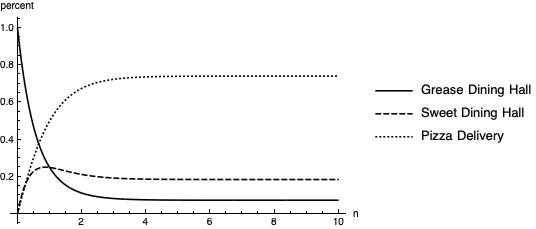
\includegraphics[width=0.5\linewidth]{3.jpg}
	\end{figure}
	where the long-term percentage approaches 7.41\% for Grease Dining Hall, 18.52\% for Sweet Dining Hall and 74.07\% for pizza delivery.
	
	\item 
	Given the data in the diagram, we have the model:
	\begin{align*}
		a_{n+1} &= 0.35 a_n + 0.1 b_n\\
		b_{n+1} &= 0.65 a_n + 0.9 b_n
	\end{align*}
	Assuming that the entire pollution is originally in Lake A, by Mathematica, the graph of the long term behavior is obtained:
	\begin{figure}[H]
		\centering
		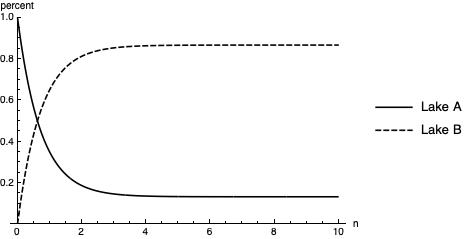
\includegraphics[width=0.5\linewidth]{4.jpg}
	\end{figure}
	where the long-term percentage approaches 13.33\% for Lake A and 86.67\% for Lake B.
	
	\item 
	Alternative 1:\\
	The reliability of the power subsystem is $R_p = 0.993$.\\
	The reliability of the communication subsystem is $R_c = 0.995 + 0.995 - 0.995 \cdot 0.995 = 0.999975$.\\
	The reliability of the landing subsystem is $R_l = (0.99 \cdot 0.999) + 0.998 - (0.99 \cdot 0.999) \cdot 0.998 = 0.999978$.\\
	The reliability of the storage subsystem is $R_s = 0.98$.\\
	The reliability of the rockets subsystem is $R_r = (0.99 \cdot 0.99) + (0.99 \cdot 0.99) - (0.99 \cdot 0.99) \cdot (0.99 \cdot 0.99) = 0.999604$.\\
	The reliablity of the system of alternative 1 is $R_{a1} = R_p \cdot R_c \cdot R_l \cdot R_s \cdot R_r = 0.993 \cdot 0.999975 \cdot 0.999978 \cdot 0.98 \cdot 0.999604 = 0.972709$.
	
	Alternative 2:\\
	The reliability of the power subsystem is $R_p = 0.998$.\\
	The reliability of the communication subsystem is $R_c = 0.995 + 0.995 - 0.995 \cdot 0.995 = 0.999975$.\\
	The reliability of the landing subsystem is $R_l = 1 - (1 - 0.99) \cdot (1 - 0.999) \cdot (1 - 0.998) = 0.999999$.\\
	The reliability of the storage subsystem is $R_s = 0.98$.\\
	The reliability of the rockets subsystem is $R_r = 1 - (1 - 0.99) \cdot (1 - 0.99) \cdot (1 - 0.99) \cdot (1 - 0.99) = 0.999999$.\\
	The reliablity of the system of alternative 1 is $R_{a2} = R_p \cdot R_c \cdot R_l \cdot R_s \cdot R_r = 0.998 \cdot 0.999975 \cdot 0.999999 \cdot 0.98 \cdot 0.999999 = 0.978014$.
	
	Since the reliability of alternative 2 is higher, I would recommend alternative 2 to NASA. The assumption is the reliability of each subsystem remains the same during the mission, which would be reasonable if the relevant technology allows.
\end{enumerate}

\end{document}

